\documentclass[../main.tex]{subfiles}
\begin{document}

\section{Estado del arte}
En esta sección se revisa el estado del arte relacionado con la segmentación de imágenes médicas, con especial atención al caso de la RM de imágenes cerebrales. Se analizan los distintos enfoques en segmentación semántica, así como las arquitecturas de redes neuronales empleadas en este trabajo: U-Net y YOLO. Asimismo, se examinan las técnicas recientes de mejora de resolución mediante redes neuronales, haciendo énfasis en el modelo FSRCNN. Esta revisión proporciona el contexto necesario para justificar las decisiones metodológicas adoptadas en el presente trabajo y permite situar la propuesta dentro del marco actual de investigación.

\subsection{Imagen por resonancia magnética}
La RM es una de las técnicas de obtención de imágenes médicas más utilizadas y seguras en la actualidad. A diferencia de otros métodos como la radiografía, la tomografía computarizada (CT), la tomografía por emisión de positrones (PET), la SPECT o el ultrasonido, la RM no utiliza radiación ionizante, lo que la hace adecuada para estudios repetidos sin riesgo para el paciente.

La RM se basa en el comportamiento de los protones de hidrógeno, 
abundantes en el cuerpo humano, cuando son expuestos a un campo magnético estático. Bajo este campo, los protones alinean su magnetización y, al aplicar una onda de radiofrecuencia, se perturban. Cuando regresan a su estado de equilibrio, emiten una señal que se registra para formar la imagen \cite{brown2014mri}. Este proceso permite generar imágenes con diferente contraste, dependiendo de tres parámetros fundamentales:

\begin{itemize}
    \item Densidad de protones ($\rho$)
    \item Tiempo de relajación T1 (spin-rejilla): cuánto tarda la 
    magnetización en volver a su equilibrio longitudinal.
    \item Tiempo de relajación T2 (spin-spin): cuánto tarda en desaparecer
    la coherencia transversal de los protones.
\end{itemize}
    
A partir de estos parámetros, se pueden generar diferentes tipos de imágenes: T1-weighted, T2-weighted y $\rho$-weighted, cada una útil para resaltar distintos tipos de tejido o anomalías \cite{Balafar2010}. Además, se emplean secuencias especializadas como FLAIR (Fluid Attenuated Inversion Recovery), que suprime el líquido cefalorraquídeo para facilitar la detección de lesiones hiperintensas periventriculares —una característica típica de la esclerosis múltiple— (ver Figura \ref{fig:flair-ms}). La secuencia FLAIR combina sensibilidad a lesiones como en T2, pero con mejor contraste en zonas cercanas a los ventrículos cerebrales \cite{bakshi2001fluid}.

\begin{figure}
    \centering
    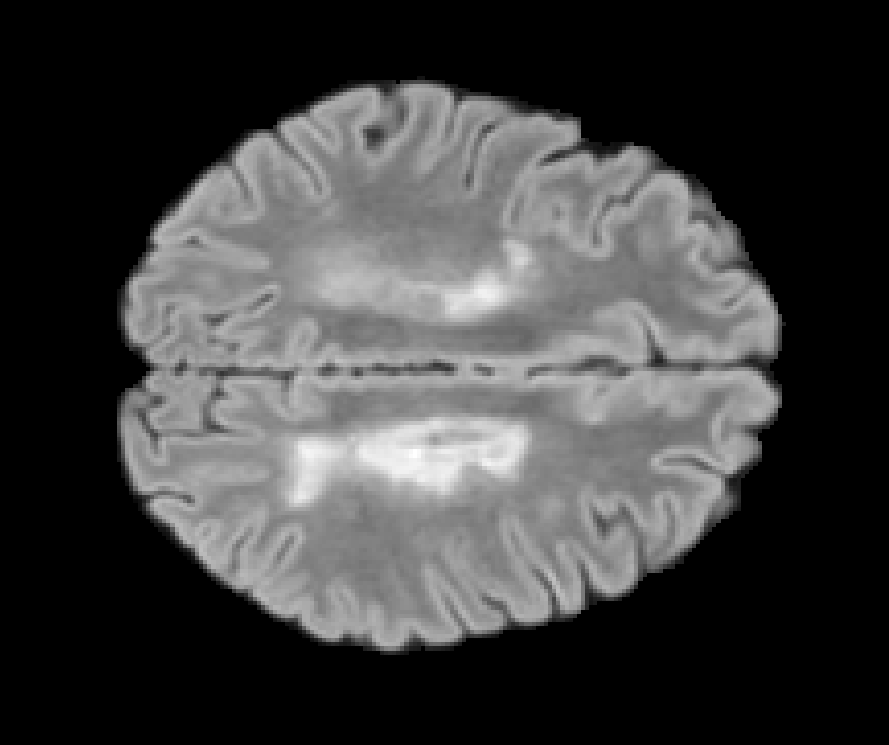
\includegraphics[width=0.5\linewidth]{imgs/arte/mri-1.png}
    \caption{Imagen FLAIR de un paciente con EM (la lesión es la zona blanca)}
    \label{fig:flair-ms}
\end{figure}

\subsection{Métodos de segmentación}
La segmentación en imágenes médicas ha evolucionado significativamente, desde métodos clásicos basados en intensidad hasta enfoques modernos de aprendizaje profundo. Esta evolución ha estado motivada por la necesidad de mejorar la precisión, robustez y automatización en la detección de estructuras y lesiones, como en el caso del cerebro en estudios de RM.

\subsubsection{Basados en intensidad}
Los métodos clásicos, como el método del valor umbral (thresholding) y las técnicas basadas en regiones, utilizan directamente los valores de intensidad de los píxeles. Un ejemplo temprano es el método de Otsu \cite{Otsu}. Aunque simples y rápidos, estos enfoques son sensibles al ruido y a la no homogeneidad de intensidad, por lo que su desempeño es limitado en imágenes complejas.

\subsubsection{Basados en regiones}
Estas técnicas identifican regiones conectadas con intensidades similares, a partir de un punto inicial. Ejemplos incluyen métodos con contornos activos localizados (LRACM) \cite{ilunga2017automatic} o análisis de simetría en 3D \cite{kermi2018fully}. Aunque más robustas que el método del valor umbral, dependen de parámetros manuales y pueden ser sensibles a la inicialización.

\subsubsection{Aprendizaje automático tradicional}
El machine learning clásico, como k-means, SVM (\textit{Support Vector Machine}) o \textit{random forests}, mejora la segmentación al utilizar características extraídas (intensidad, textura, forma). Métodos como los super-vóxeles combinados con \textit{random forest} \cite{SOLTANINEJAD201869}, o modelos semi-supervisados con restricciones espaciales \cite{8481468}, resultan en mejores segmentaciónes. Sin
embargo, muchos de estos enfoques siguen dependiendo de la ingeniería manual de características y pueden ser computacionalmente intensivos.

\subsubsection{Aprendizaje profundo}
Con la llegada del aprendizaje profundo, la segmentación alcanzó nuevos niveles de precisión. Las redes convolucionales (CNN) permiten aprender directamente las características relevantes desde los datos, reduciendo la necesidad de diseño manual:

\begin{itemize}
    \item 2D CNNs como las de Pereira et al. \cite{7426413} y Havaei et al. \cite{HAVAEI201718} mostraron avances notables, aunque limitados por la falta de contexto tridimensional.
    \item Modelos 2.5D abordan este problema procesando múltiples cortes adyacentes \cite{MILLETARI201792,wang2019automatic}.
    \item Redes 3D como las de Myronenko \cite{myronenko2018mri} o Baid et al. \cite{baid2020novel} permiten un análisis volumétrico completo, aunque requieren más recursos computacionales.

\end{itemize}
    
\subsubsection{Enfoques híbridos}
Los métodos híbridos combinan lo mejor de varios enfoques:
\begin{itemize}
    \item Aprendizaje profundo junto con aprendizaje automático tradicional, como por ejemplo CNN con \textit{Conditional Random Field } (CRF) \cite{kamnitsas2017efficient}.
    \item Segmentación basada en contornos junto con aprendizaje automático, como modelos que combinan \textit{random forests} con contornos activos \cite{ma2018concatenated}.
    \item Metaheurísticas junto con \textit{clustering}, como \textit{Fuzzy C-Means} (FCM) con algoritmos evolutivos \cite{pham2019multi}.
 
\end{itemize}

%\begin{table}[htbp]
%\centering
%\caption{Comparativa de métodos de segmentación en imágenes %médicas}
%\label{tab:comparativa_metodos}
%\begin{tabularx}{\textwidth}{@{}p{2.8cm} p{3.2cm} X X@{}}
%\toprule
%\textbf{Enfoque} & \textbf{Tipo de datos} & \textbf{Ventajas} %& \textbf{Limitaciones} \\
%\midrule
%Basados en intensidad & Valores de intensidad de píxel & Simplicidad y rapidez & Muy sensible al ruido y a la falta de %homogeneidad en la intensidad \\
%\addlinespace
%Basados en regiones & Regiones conectadas por similitud de intensidad & Mejor delimitación espacial & Dependencia de %parámetros iniciales como semillas o umbrales \\
%\addlinespace
%Aprendizaje automático tradicional & Características extraídas %(intensidad, textura, forma) & Mayor precisión que métodos clásicos & Requiere ingeniería manual de características y %datos etiquetados \\
%\addlinespace
%Aprendizaje profundo (2D, 2.5D, 3D) & Imágenes crudas en %distintos planos & Alto rendimiento y aprendizaje automático de características relevantes & Alta demanda computacional y %necesidad de grandes cantidades de datos \\
%\addlinespace
%Enfoques híbridos & Combinación de métodos anteriores & Mejora la precisión y la robustez & Complejidad del diseño y %necesidad de ajustar múltiples componentes \\
%\bottomrule
%\end{tabularx}
%\end{table}


\subsection{Super-resolución en imágenes MRI}
Los algoritmos de super-resolución se basan en un modelo general de adquisición que describe cómo una imagen de alta resolución ideal $X$ se degrada durante el proceso de captura para dar lugar a una secuencia de imágenes de baja resolución $Y_kY_k$. Este modelo, ampliamente aceptado en la literatura, se puede expresar como:

\begin{equation}
    Y_k=D_kB_kG_kX+V_k
\end{equation}

donde $G_k$ representa la transformación geométrica (como el movimiento del paciente), $B_k$ es el operador de desenfoque asociado a la adquisición de las propias imágenes RM (PSF), $D_k$ es el operador de submuestreo, y $V_k$ representa el ruido aditivo, generalmente gaussiano. Para simplificar, esta expresión también puede escribirse de forma compacta como $Y_k=W_kX+V_kY_k = W_kX+V_k$, donde $W_k$ es el operador global que resume todos los efectos degradantes. La tarea de SR consiste en invertir este modelo para estimar la imagen X, lo cual constituye un problema mal planteado, razón por la cual se recurre a técnicas de optimización~\cite{sr_systematic_r}.

A partir de este modelo, se han propuesto diversos enfoques para invertir el proceso y estimar $X$. Entre ellos destacan los métodos basados en \textit{Iterative Back-Projection}, técnicas deterministas con regularización (como mínimos cuadrados o variación total), enfoques estadísticos bayesianos como el estimador MAP, y métodos geométricos como la proyección en conjuntos convexos (POCS) \cite{sr_systematic_r}.
Todos ellos comparten la necesidad de incorporar información a priori para compensar el carácter mal planteado del problema.

Sin embargo, estos métodos tradicionales presentan limitaciones. En primer lugar, dependen fuertemente de una estimación precisa del movimiento entre cortes o adquisiciones ($G_k$), lo cual resulta problemático en presencia de movimientos impredecibles o deformaciones anatómicas sutiles. Además, muchos algoritmos asumen que el perfil de desenfoque (PSF) es conocido y constante, lo cual rara vez se cumple en escenarios clínicos. Por otro lado, el ruido en RM no siempre se ajusta al modelo gaussiano simple utilizado en estas formulaciones, y la variabilidad del contraste entre sujetos también dificulta la generalización. Así pues, aunque estos métodos son usados, requieren parámetros cuya elección puede tener un mayor impacto en el resultado que el propio método seleccionado \cite{sr_systematic_r}, lo que puede limitar su aplicabilidad práctica en entornos clínicos. Además, su capacidad para recuperar estructuras finas, especialmente en el contexto de lesiones pequeñas o bordes difusos como ocurre en la esclerosis múltiple, puede verse comprometida por la sensibilidad a errores de registración o la imposición de regularizadores demasiado restrictivos.

En vista de las limitaciones de los métodos clásicos de super-resolución en resonancia magnética, el uso de redes neuronales profundas ha emergido como una alternativa eficaz y flexible para mejorar la resolución espacial sin necesidad de suposiciones estrictas sobre el modelo de adquisición. 
Por un lado, técnicas como SMORE (Self Super-Resolution) han demostrado su aplicabilidad directa en imágenes clínicas reales, utilizando redes del estado del arte como EDSR para generar datos de entrenamiento directamente a partir de las propias imágenes adquiridas \cite{9253710}. Esto elimina la necesidad de conjuntos de datos externos de entrenamiento y permite preservar detalles patológicos mientras se mejora la visualización en múltiples contextos clínicos, como esclerosis múltiple, remodelado cardíaco o segmentación ventricular \cite{ZHAO2019132}. Por otro lado, arquitecturas más complejas como GAN-CPCE y GAN-CIRCLE, han mostrado resultados prometedores al ser usadas en imágenes de resonancia magnética, alcanzando mejoras cuantificables en métricas como PSNR y SSIM \cite{lyu2018super}. Estas redes combinan estrategias de entrenamiento para producir imágenes detalladas con bordes más definidos, lo cual es especialmente útil en tareas de diagnóstico estructural. En conjunto, estas propuestas demuestran que los enfoques basados en aprendizaje profundo no solo superan en calidad a las técnicas tradicionales o basadas en interpolación. Esto refuerza la elección de redes neuronales profundas como método para abordar la super-resolución en este trabajo.
\end{document}